
\documentclass[border=8pt, multi, tikz]{standalone} 
\usepackage{import}
\subimport{../layers/}{init}
\usetikzlibrary{positioning}
\usetikzlibrary{3d} %for including external image 

\def\ConvColor{rgb:yellow,5;red,2.5;white,5}
\def\ConvReluColor{rgb:yellow,5;red,5;white,5}
\def\PoolColor{rgb:red,1;black,0.3}
\def\UnpoolColor{rgb:blue,2;green,1;black,0.3}
\def\FcColor{rgb:blue,5;red,2.5;white,5}
\def\FcReluColor{rgb:blue,5;red,5;white,4}
\def\SoftmaxColor{rgb:magenta,5;black,7}   

\newcommand{\copymidarrow}{\tikz \draw[-Stealth,line width=0.8mm,draw={rgb:blue,4;red,1;green,1;black,3}] (-0.3,0) -- ++(0.3,0);}

\begin{document}
\begin{tikzpicture}
\tikzstyle{connection}=[ultra thick,every node/.style={sloped,allow upside down},draw=\edgecolor,opacity=0.7]
\tikzstyle{copyconnection}=[ultra thick,every node/.style={sloped,allow upside down},draw={rgb:blue,4;red,1;green,1;black,3},opacity=0.7]

\node[canvas is zy plane at x=0] (temp) at (-3,0,0) {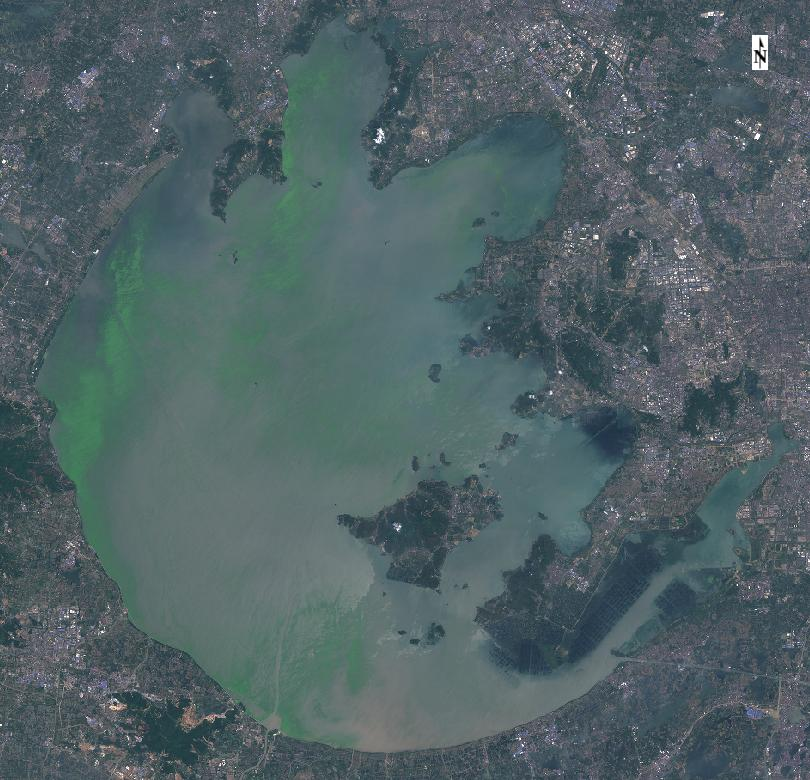
\includegraphics[width=14cm,height=14cm]{taihu_on_flowchart.jpg}};

\pic[shift={(0,0,0)}] at (0,0,0) 
    {Box={
        name=e1c1,
        caption= ,
        xlabel={{64, }},
        zlabel=256,
        fill=\ConvColor,
        height=64,
        width=2,
        depth=64
        }
    };

\pic[shift={(0,0,0)}] at (e1c1-east) 
    {Box={
        name=e1c2,
        caption= ,
        xlabel={{64, }},
        zlabel=256,
        fill=\ConvColor,
        height=64,
        width=2,
        depth=64
        }
    };

\pic[shift={ (0,0,0) }] at (e1c2-east) 
    {Box={
        name=e1p1,
        caption= ,
        fill=\PoolColor,
        opacity=0.5,
        height=48,
        width=1,
        depth=48
        }
    };

\pic[shift={(3,0,0)}] at (e1p1-east) 
    {Box={
        name=e2c1,
        caption= ,
        xlabel={{128, }},
        zlabel=128,
        fill=\ConvColor,
        height=48,
        width=4,
        depth=48
        }
    };

\draw [connection]  (e1p1-east)    -- node {\midarrow} (e2c1-west);

\pic[shift={(0,0,0)}] at (e2c1-east) 
    {Box={
        name=e2c2,
        caption= ,
        xlabel={{128, }},
        zlabel=128,
        fill=\ConvColor,
        height=48,
        width=4,
        depth=48
        }
    };

\pic[shift={ (0,0,0) }] at (e2c2-east) 
    {Box={
        name=e2p1,
        caption= ,
        fill=\PoolColor,
        opacity=0.5,
        height=36,
        width=1,
        depth=36
        }
    };

\pic[shift={(2,0,0)}] at (e2p1-east) 
    {Box={
        name=e3c1,
        caption= ,
        xlabel={{256, }},
        zlabel=64,
        fill=\ConvColor,
        height=36,
        width=6,
        depth=36
        }
    };

\draw [connection]  (e2p1-east)    -- node {\midarrow} (e3c1-west);

\pic[shift={(0,0,0)}] at (e3c1-east) 
    {Box={
        name=e3c2,
        caption= ,
        xlabel={{256, }},
        zlabel=64,
        fill=\ConvColor,
        height=36,
        width=6,
        depth=36
        }
    };

\pic[shift={(0,0,0)}] at (e3c2-east) 
    {Box={
        name=e3c3,
        caption= ,
        xlabel={{256, }},
        zlabel=64,
        fill=\ConvColor,
        height=36,
        width=6,
        depth=36
        }
    };

\pic[shift={ (0,0,0) }] at (e3c3-east) 
    {Box={
        name=e3p1,
        caption= ,
        fill=\PoolColor,
        opacity=0.5,
        height=28,
        width=1,
        depth=28
        }
    };

\pic[shift={(1.5,0,0)}] at (e3p1-east) 
    {Box={
        name=e4c1,
        caption= ,
        xlabel={{512, }},
        zlabel=32,
        fill=\ConvColor,
        height=28,
        width=8,
        depth=28
        }
    };

\draw [connection]  (e3p1-east)    -- node {\midarrow} (e4c1-west);

\pic[shift={(0,0,0)}] at (e4c1-east) 
    {Box={
        name=e4c2,
        caption= ,
        xlabel={{512, }},
        zlabel=32,
        fill=\ConvColor,
        height=28,
        width=8,
        depth=28
        }
    };

\pic[shift={(0,0,0)}] at (e4c2-east) 
    {Box={
        name=e4c3,
        caption= ,
        xlabel={{512, }},
        zlabel=32,
        fill=\ConvColor,
        height=28,
        width=8,
        depth=28
        }
    };

\pic[shift={ (0,0,0) }] at (e4c3-east) 
    {Box={
        name=e4p1,
        caption= ,
        fill=\PoolColor,
        opacity=0.5,
        height=20,
        width=1,
        depth=20
        }
    };

\pic[shift={(1.5,0,0)}] at (e4p1-east) 
    {Box={
        name=e5c1,
        caption= ,
        xlabel={{1024, }},
        zlabel=16,
        fill=\ConvColor,
        height=20,
        width=10,
        depth=20
        }
    };

\draw [connection]  (e4p1-east)    -- node {\midarrow} (e5c1-west);

\pic[shift={(0,0,0)}] at (e5c1-east) 
    {Box={
        name=e5c2,
        caption= ,
        xlabel={{1024, }},
        zlabel=16,
        fill=\ConvColor,
        height=20,
        width=10,
        depth=20
        }
    };

\pic[shift={(0,0,0)}] at (e5c2-east) 
    {Box={
        name=e5c3,
        caption= ,
        xlabel={{1024, }},
        zlabel=16,
        fill=\ConvColor,
        height=20,
        width=10,
        depth=20
        }
    };

\pic[shift={ (0,0,0) }] at (e5c3-east) 
    {Box={
        name=e5p1,
        caption= ,
        fill=\PoolColor,
        opacity=0.5,
        height=15,
        width=1,
        depth=15
        }
    };

\pic[shift={ (1,0,0) }] at (e5p1-east) 
    {Box={
        name=d1p1,
        caption= ,
        fill=\UnpoolColor,
        opacity=0.5,
        height=20,
        width=1,
        depth=20
        }
    };

\draw [connection]  (e5p1-east)    -- node {\midarrow} (d1p1-west);

\pic[shift={ (0,0,0) }] at (d1p1-east) 
    {RightBandedBox={
        name=d1c1,
        caption= ,
        xlabel={{ 1024, }},
        zlabel=16,
        fill={rgb:white,1;black,3},
        bandfill={rgb:white,1;black,2},
        opacity=0.2,
        height=20,
        width=10,
        depth=20
        }
    };

\pic[shift={(0,0,0)}] at (d1c1-east) 
    {Box={
        name=d1c2,
        caption= ,
        xlabel={{1024, }},
        zlabel=16,
        fill=\ConvColor,
        height=20,
        width=10,
        depth=20
        }
    };

\pic[shift={ (0,0,0) }] at (d1c2-east) 
    {RightBandedBox={
        name=d1c3,
        caption= ,
        xlabel={{ 1024, }},
        zlabel=16,
        fill={rgb:white,1;black,3},
        bandfill={rgb:white,1;black,2},
        opacity=0.2,
        height=20,
        width=10,
        depth=20
        }
    };

\pic[shift={ (1.5,0,0) }] at (d1c3-east) 
    {Box={
        name=d2p1,
        caption= ,
        fill=\UnpoolColor,
        opacity=0.5,
        height=28,
        width=1,
        depth=28
        }
    };

\draw [connection]  (d1c3-east)    -- node {\midarrow} (d2p1-west);

\pic[shift={ (0,0,0) }] at (d2p1-east) 
    {RightBandedBox={
        name=d2c1,
        caption= ,
        xlabel={{ 512, }},
        zlabel=32,
        fill={rgb:white,1;black,3},
        bandfill={rgb:white,1;black,2},
        opacity=0.2,
        height=28,
        width=8,
        depth=28
        }
    };

\pic[shift={(0,0,0)}] at (d2c1-east) 
    {Box={
        name=d2c2,
        caption= ,
        xlabel={{512, }},
        zlabel=32,
        fill=\ConvColor,
        height=28,
        width=8,
        depth=28
        }
    };

\pic[shift={ (0,0,0) }] at (d2c2-east) 
    {RightBandedBox={
        name=d2c3,
        caption= ,
        xlabel={{ 512, }},
        zlabel=32,
        fill={rgb:white,1;black,3},
        bandfill={rgb:white,1;black,2},
        opacity=0.2,
        height=28,
        width=8,
        depth=28
        }
    };

\pic[shift={ (2,0,0) }] at (d2c3-east) 
    {Box={
        name=d3p1,
        caption= ,
        fill=\UnpoolColor,
        opacity=0.5,
        height=36,
        width=1,
        depth=36
        }
    };

\draw [connection]  (d2c3-east)    -- node {\midarrow} (d3p1-west);

\pic[shift={ (0,0,0) }] at (d3p1-east) 
    {RightBandedBox={
        name=d3c1,
        caption= ,
        xlabel={{ 256, }},
        zlabel=64,
        fill={rgb:white,1;black,3},
        bandfill={rgb:white,1;black,2},
        opacity=0.2,
        height=36,
        width=6,
        depth=36
        }
    };

\pic[shift={(0,0,0)}] at (d3c1-east) 
    {Box={
        name=d3c2,
        caption= ,
        xlabel={{256, }},
        zlabel=64,
        fill=\ConvColor,
        height=36,
        width=6,
        depth=36
        }
    };

\pic[shift={ (0,0,0) }] at (d3c2-east) 
    {RightBandedBox={
        name=d3c3,
        caption= ,
        xlabel={{ 256, }},
        zlabel=64,
        fill={rgb:white,1;black,3},
        bandfill={rgb:white,1;black,2},
        opacity=0.2,
        height=36,
        width=6,
        depth=36
        }
    };

\pic[shift={ (2,0,0) }] at (d3c3-east) 
    {Box={
        name=d4p1,
        caption= ,
        fill=\UnpoolColor,
        opacity=0.5,
        height=48,
        width=1,
        depth=48
        }
    };

\draw [connection]  (d3c3-east)    -- node {\midarrow} (d4p1-west);

\pic[shift={ (0,0,0) }] at (d4p1-east) 
    {RightBandedBox={
        name=d4c1,
        caption= ,
        xlabel={{ 256, }},
        zlabel=64,
        fill={rgb:white,1;black,3},
        bandfill={rgb:white,1;black,2},
        opacity=0.2,
        height=48,
        width=4,
        depth=48
        }
    };

\pic[shift={(0,0,0)}] at (d4c1-east) 
    {Box={
        name=d4c2,
        caption= ,
        xlabel={{256, }},
        zlabel=64,
        fill=\ConvColor,
        height=48,
        width=4,
        depth=48
        }
    };

\pic[shift={ (2,0,0) }] at (d4c2-east) 
    {Box={
        name=d5p1,
        caption= ,
        fill=\UnpoolColor,
        opacity=0.5,
        height=64,
        width=1,
        depth=64
        }
    };

\draw [connection]  (d4c2-east)    -- node {\midarrow} (d5p1-west);

\pic[shift={ (0,0,0) }] at (d5p1-east) 
    {RightBandedBox={
        name=d5c1,
        caption= ,
        xlabel={{ 256, }},
        zlabel=64,
        fill={rgb:white,1;black,3},
        bandfill={rgb:white,1;black,2},
        opacity=0.2,
        height=64,
        width=2,
        depth=64
        }
    };

\pic[shift={(0,0,0)}] at (d5c1-east) 
    {Box={
        name=d5c2,
        caption= ,
        xlabel={{256, }},
        zlabel=64,
        fill=\ConvColor,
        height=64,
        width=2,
        depth=64
        }
    };

\pic[shift={(3,0,0)}] at (d5c2-east) 
    {Box={
        name=soft1,
        caption=SOFT,
        xlabel={{" ","dummy"}},
        zlabel=10,
        fill=\SoftmaxColor,
        opacity=0.8,
        height=64,
        width=1,
        depth=64
        }
    };

\draw [connection]  (d5c2-east)    -- node {\midarrow} (soft1-west);

\end{tikzpicture}
\end{document}
